\section{Data Analysis / Processing}
This section covers processing and analysis of acquired data. All data processing is performed using MATLAB. 

%maybe something on filtering if we end up doing that
\subsection{Filtering}
%Butterworth filtering of the gyroscope measurements
%Filtering has been implemented in the form of a low pass third order Butterworth filter with a cut off frequency at 25Hz. Since measurement are 
The spectral density of gyroscope data have been analysed to investigate frequencies of interest. From the Fourier transform (FT) of gyroscope data (see \figref{fig:gyroFFTPlot}) it can be observed that frequencies over 10Hz contain very little information. To avoid possible noise and artefacts a low pass third order Butterworth filter have been implemented with a cut off frequency at 25Hz. %This filter order and cut off frequency is decided \textbf{??}

\begin{figure}[H]
	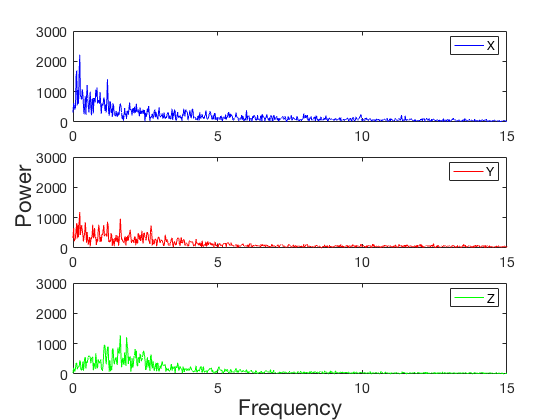
\includegraphics[width=.6\textwidth]{figures/gyroFFTPlot}
	\caption{The power spectral density of gyroscope data from the left leg of one subject.}
	\label{fig:gyroFFTPlot}  %<--remember LABEL!
\end{figure}



%MATLAB alignment GUI description
\subsection{Data Alignment}
Because the measurements from the FSRs are run on an Arduino, and the gyroscopes run through a Shimmer Sensing developed script for MATLAB, the timing for the measurements are run differently. In order to analyse FSR data to the corresponding time for gyroscope data a data alignment GUI have been developed in MATLAB. The implemented alignment program is a simple GUI which creates a plot where different channels from the six FSRs and six DoFs from the gyroscopes (three for each on each leg) can be shown or hidden. Additionally each channel can be translated left or right. This enables to align data from the FSRs to the gyroscopes, based on a spike in measurements caused by a small jump subjects will be asked to perform before and after performance of Pinan Nidan. An example of the alignment GUI can be seen in \figref{fig:alignGUI}.

\begin{figure}[H]
	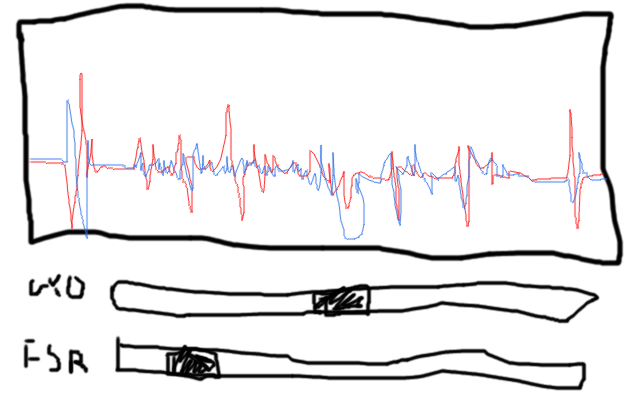
\includegraphics[width=.6\textwidth]{figures/alignGUI}
	\caption{The alignment GUI showing a selected number of channels from the FSRs and gyroscopes. All channels can be translated in order to align timestamps for the FSR measurements to timestamps for the gyroscopes.}
	\label{fig:alignGUI}  %<--remember LABEL!
\end{figure}


\subsection{Calculation of movement scores}

For calculating a movement score four separate scores will be calculated; COP, length, span and frequency distribution. COP is a calculation of the estimated COP for a test subject on a plane. The length is calculated on the path of the moving COP during recording. Span is a calculation of the area in which the COP has travelled. Frequency distribution is a measure for the gyroscope frequencies measured during recordings. Here, low frequencies (2/3 of the frequency spectrum from 0 to 5Hz) are an expression for stable movements, and high frequencies (the last 1/3 of the frequency spectrum from 0 to 5Hz) are an expression for less stable movements. This separation of low and high frequencies is based on when the frequency distribution deviated less than 5\% of mean for individual subject.

\subsubsection{Calculation of Centre of Pressure}
%method for calculation of COP 
%MATLAB COP code description
The COP (check for prior use of abbreviation) calculation consists of two simple equations to find the displacement of balance in the X and Y directions. To ensure the calculated values are unrelated to the weight of the test subject, but solely describes the displacement of balance, each calculation of the pressure distribution will be divided by the overall pressure placed on all sensors. The COP\lowercase{x} equation finds the distribution of weight between the two feet, whereas the COP\lowercase{y} equation describes the distribution between the sensors on the front and back of the foot. To compensate for the number of sensors on the front and back of the foot, in addition to the displacement of these sensors in relation to each other, a weight will be added to the pressure readings.
The COP calculations for X and Y directions follow \eqref{eq:COPx} and \eqref{eq:COPy}:

\begin{equation}
COP_x(i) =  \frac{\sum_{i=1}^{3}P_i W_i - \sum_{i=4}^{6}P_i W_i}{\sum_{i=1}^{6}P_i W_i}
\end{equation} \label{eq:COPx}

\begin{equation}
COP_y(i) =  \frac{\sum(P_3 W_3 + P_6 W_6) - \sum(P_1 W_1+P_2 W_2+P_4 W_4+P_5 W_5)}{\sum_{i=1}^{6}P_i W_i}
\end{equation} \label{eq:COPy}



%method for calculating scores based on calculated COP and gyroscope data

\subsubsection{Calculation of length measure}
The length of the COP outcomes was calculated and divided by the length (L) of the recorded data, so the outcome measure described the mean COP change between each sample. To ensure this measure had an effect on the final score it was multiplied by a factor of 10. The length was calculated individually for X and Y directions for later use in score calculation (see \eqref{eq:length}).

\begin{equation}
	Length_{x,y} = \frac{\sum_{i=1}^{L-1}\sqrt{(COP_{x,y} (i+1)-COP_{x,y} (i))^2}}{L} * 10
\end{equation}




\subsubsection{Calculation of span measure}





\subsubsection{Calculation of frequency distribution}




